\documentclass[11pt]{article}
\usepackage{graphicx}
\usepackage{geometry}
\geometry{margin=0.5in}
\usepackage{amsmath}
\usepackage{booktabs}
\usepackage{siunitx}
\sisetup{detect-all}

\title{EE577B HW2 Part C: Testbench Analysis and Verification}
\author{}
\date{}

\begin{document}
\maketitle

\vspace{-50pt}
\section*{Testbench configuration}
Clock frequency is \SI{100}{MHz} with period \SI{10}{ns}. Sampling occurs on every negative edge at times \SI{5}{ns}, \SI{15}{ns}, \SI{25}{ns}, and so on. The shared reset signal \texttt{rst} is used by all four DFFs which internally interpret polarity and synchrony as required by the specification:
\begin{center}
\begin{tabular}{@{}llll@{}}
\toprule
Module & Reset mechanism & Reset polarity & Data enable polarity \\
\midrule
\texttt{dff\_alpha} & Synchronous & Active HIGH & Active HIGH \\
\texttt{dff\_beta}  & Asynchronous & Active HIGH & Active LOW \\
\texttt{dff\_gamma} & Synchronous & Active LOW  & Active HIGH \\
\texttt{dff\_delta} & Asynchronous & Active LOW  & Active LOW \\
\bottomrule
\end{tabular}
\end{center}

The testbench asserts reset for five clock cycles at the beginning as follows. From \SI{0}{ns} to \SI{50}{ns} \texttt{rst} is \texttt{1} which asserts alpha and beta. From \SI{50}{ns} to \SI{100}{ns} \texttt{rst} is \texttt{0} which asserts gamma and delta. After \SI{100}{ns} the stimulus drives explicit scenarios for functional coverage. Console timestamps provided in picoseconds have been interpreted in nanoseconds for readability.

\section*{Waveforms}

        \begin{figure}[h!]
            \centering 
            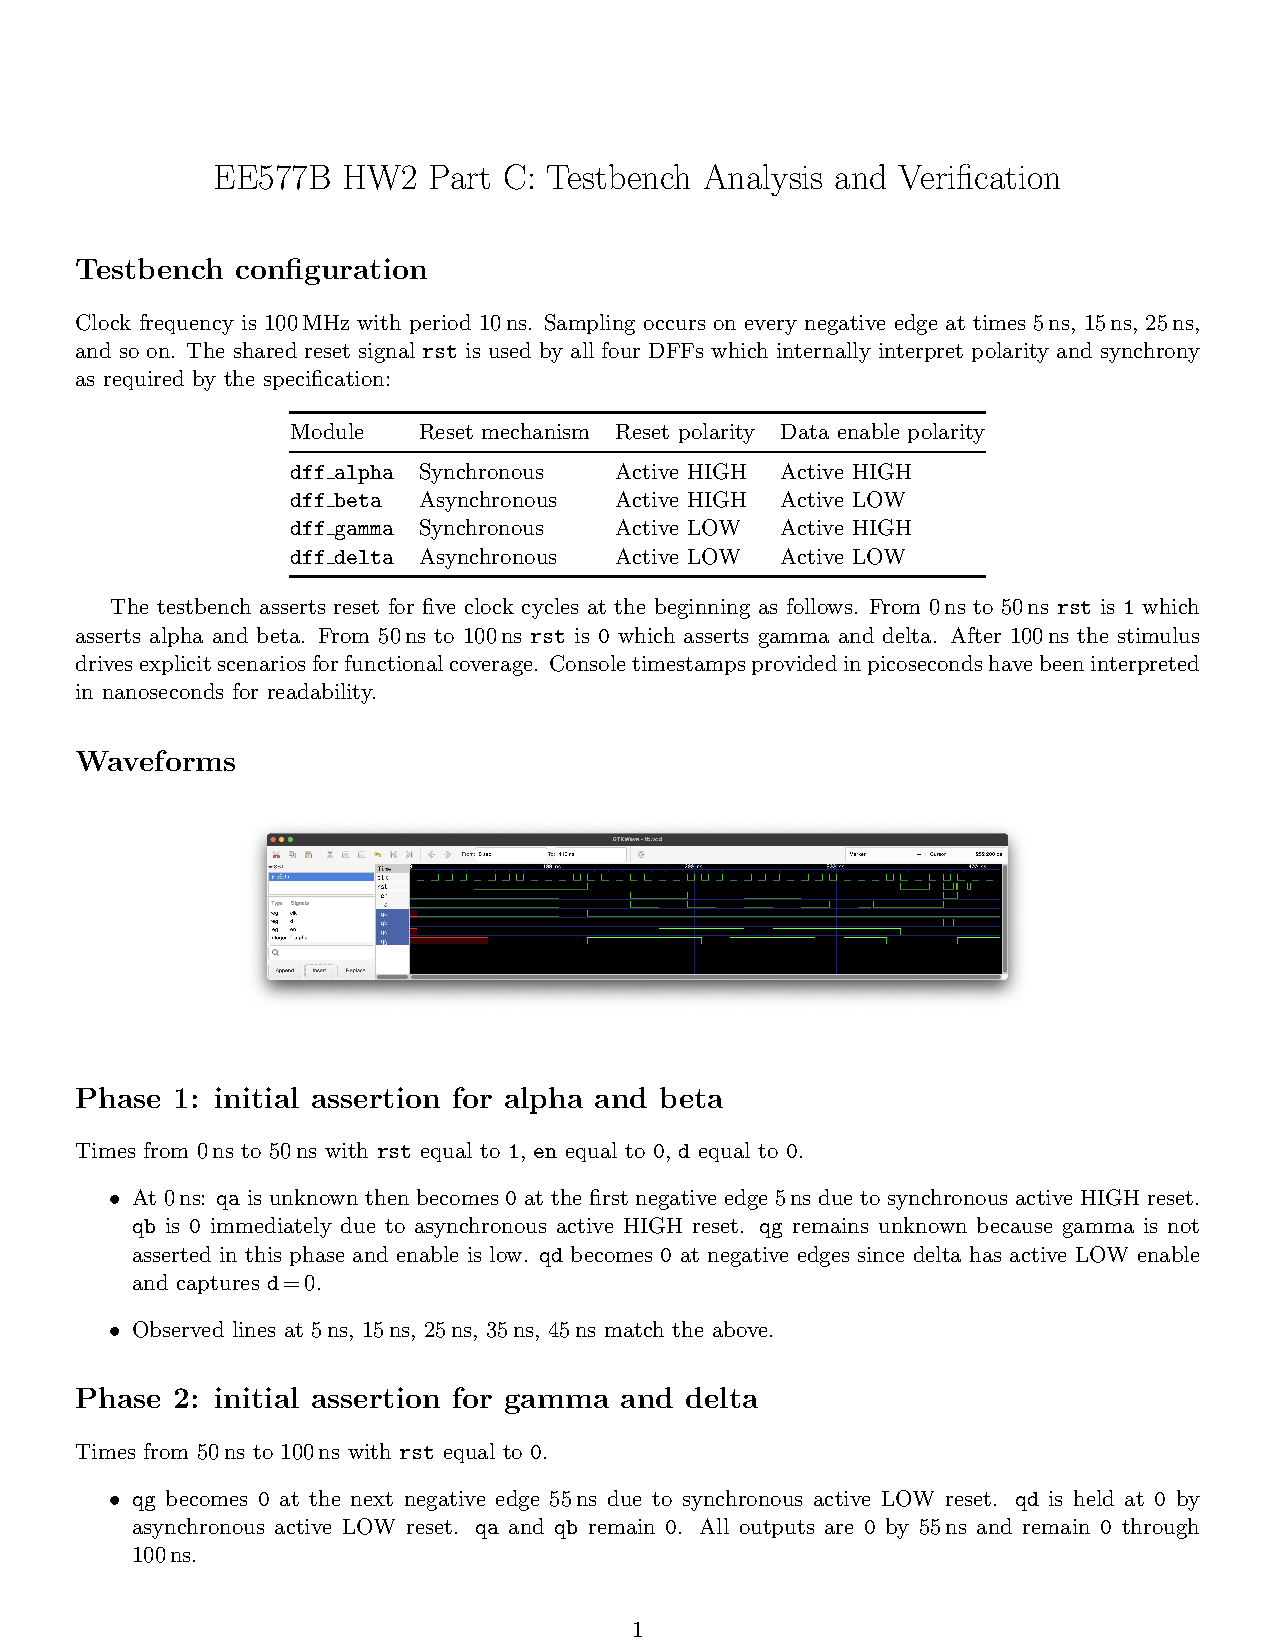
\includegraphics[width=0.7\textwidth]{C_DFF.png}
        \end{figure}

\section*{Phase 1: initial assertion for alpha and beta}
Times from \SI{0}{ns} to \SI{50}{ns} with \texttt{rst} equal to \texttt{1}, \texttt{en} equal to \texttt{0}, \texttt{d} equal to \texttt{0}.
\begin{itemize}
  \item At \SI{0}{ns}: \texttt{qa} is unknown then becomes \texttt{0} at the first negative edge \SI{5}{ns} due to synchronous active HIGH reset. \texttt{qb} is \texttt{0} immediately due to asynchronous active HIGH reset. \texttt{qg} remains unknown because gamma is not asserted in this phase and enable is low. \texttt{qd} becomes \texttt{0} at negative edges since delta has active LOW enable and captures \texttt{d}\,=\,0.
  \item Observed lines at \SI{5}{ns}, \SI{15}{ns}, \SI{25}{ns}, \SI{35}{ns}, \SI{45}{ns} match the above.
\end{itemize}

\section*{Phase 2: initial assertion for gamma and delta}
Times from \SI{50}{ns} to \SI{100}{ns} with \texttt{rst} equal to \texttt{0}.
\begin{itemize}
  \item \texttt{qg} becomes \texttt{0} at the next negative edge \SI{55}{ns} due to synchronous active LOW reset. \texttt{qd} is held at \texttt{0} by asynchronous active LOW reset. \texttt{qa} and \texttt{qb} remain \texttt{0}. All outputs are \texttt{0} by \SI{55}{ns} and remain \texttt{0} through \SI{100}{ns}.
\end{itemize}

\section*{Alpha sanity capture}
Times \SI{105}{ns} to \SI{120}{ns} with \texttt{rst} deasserted for alpha by setting \texttt{rst} equal to \texttt{0}, and with \texttt{en} equal to \texttt{1}, \texttt{d} equal to \texttt{1} prior to a negative edge.
\begin{itemize}
  \item At \SI{105}{ns} \texttt{qa} becomes \texttt{1}. This proves correct operation of alpha with synchronous active HIGH reset and active HIGH enable.
\end{itemize}

\section*{Gamma sanity capture}
Times \SI{125}{ns} to \SI{140}{ns} with \texttt{rst} deasserted for gamma by setting \texttt{rst} equal to \texttt{1}, and with \texttt{en} equal to \texttt{1}, \texttt{d} equal to \texttt{1} prior to a negative edge.
\begin{itemize}
  \item At \SI{125}{ns} \texttt{qg} becomes \texttt{1}. This proves correct operation of gamma with synchronous active LOW reset and active HIGH enable. In the same window alpha is returned to reset because \texttt{rst} is \texttt{1} which is the active level for alpha.
\end{itemize}

\section*{Exhaustive enable and data combinations}
A neutral region is maintained by holding \texttt{rst} at the deasserted level for all four modules and cycling through all \((\texttt{en},\texttt{d})\) pairs.
\begin{itemize}
  \item When \texttt{en} equals \texttt{1}, alpha and gamma capture \texttt{d} on negative edges while beta and delta hold their previous values. This behavior is visible at \SIrange{205}{235}{ns} and again later.
  \item When \texttt{en} equals \texttt{0}, beta and delta capture \texttt{d} on negative edges while alpha and gamma hold. This behavior is visible at \SI{175}{ns}, \SI{205}{ns}, \SI{235}{ns}, and subsequent repetitions.
\end{itemize}

\section*{Data timing relative to the sampling edge}
\begin{itemize}
  \item At \SI{324}{ns} and \SI{325}{ns} the stimulus changes \texttt{d} just before a negative edge then just after a negative edge. Values are captured only at the negative edge as expected. The capture one nanosecond before the edge is effective at the next negative edge. The change one nanosecond after the edge is not visible until the following negative edge.
\end{itemize}

\section*{Synchronous reset demonstrations}
\begin{itemize}
  \item For alpha with synchronous active HIGH reset, asserting \texttt{rst} equal to \texttt{1} across a negative edge returns \texttt{qa} to \texttt{0} at that edge. This is observed in the region around \SI{345}{ns} to \SI{370}{ns}.
  \item For gamma with synchronous active LOW reset, asserting \texttt{rst} equal to \texttt{0} across a negative edge returns \texttt{qg} to \texttt{0} at that edge. This is observed in the same region when \texttt{rst} is driven low.
\end{itemize}

\section*{Asynchronous reset demonstrations}
\begin{itemize}
  \item For beta with asynchronous active HIGH reset, a mid cycle assertion of \texttt{rst} equal to \texttt{1} forces \texttt{qb} to \texttt{0} immediately without waiting for a clock edge. The console shows \texttt{qb} equal to \texttt{1} at \SI{375}{ns} followed by \texttt{qb} equal to \texttt{0} when \texttt{rst} is pulsed at \SI{382}{ns}.
  \item For delta with asynchronous active LOW reset, a mid cycle assertion of \texttt{rst} equal to \texttt{0} forces \texttt{qd} to \texttt{0} immediately. This is visible in the region around \SI{392}{ns}.
\end{itemize}

\section*{Verification summary}
\begin{itemize}
  \item Initial five cycle assertions verify both reset polarities at the beginning of simulation.
  \item Alpha and gamma captures with \texttt{en} equal to \texttt{1} and \texttt{d} equal to \texttt{1} confirm synchronous operation and correct polarity handling.
  \item Exhaustive \((\texttt{en},\texttt{d})\) combinations demonstrate enable polarity for all modules.
  \item Timing checks around the negative edge confirm edge aligned sampling.
  \item Synchronous resets take effect only on the next negative edge. Asynchronous resets take effect immediately.
\end{itemize}

\end{document}
